\documentclass[aip,jcp,amsmath,amssymb,reprint]{revtex4-1}

\usepackage{graphicx}
\usepackage{booktabs}
\usepackage[utf8]{inputenc}
\usepackage[T1]{fontenc}
\usepackage{mathptmx}
\usepackage{etoolbox}
% generated by qbscreen/make_numbers_v6.py — do not edit
\newcommand{\AmineErr}{0.05}
\newcommand{\AnisoCellMax}{7.4}
\newcommand{\AnisoRowMax}{3.11}
\newcommand{\AnisoRowMin}{0.76}
\newcommand{\BornRadius}{2.81}
\newcommand{\CoulHi}{0.05}
\newcommand{\CoulLo}{0.03}
\newcommand{\Dcontact}{-843}
\newcommand{\DeltaMAOhi}{1.44}
\newcommand{\DeltaMAOlo}{1.41}
\newcommand{\DeltaMAOsub}{0.91}
\newcommand{\DeltaMAOsubHi}{0.99}
\newcommand{\DeltaMAOsubLo}{0.86}
\newcommand{\DeltaMaxHi}{0.82}
\newcommand{\DeltaMaxLo}{0.58}
\newcommand{\DeltaMaxPHi}{0.86}
\newcommand{\DeltaMaxPLo}{0.62}
\newcommand{\DeltaSiteHi}{2.00}
\newcommand{\DeltaSiteLo}{0.49}
\newcommand{\DeltaToThr}{0.41}
\newcommand{\EamExp}{1.30}
\newcommand{\Econtact}{-26}
\newcommand{\EflMAOA}{-159}
\newcommand{\EflMAOB}{-167}
\newcommand{\EmFreeA}{-211}
\newcommand{\EoneCap}{0.29}
\newcommand{\EoneShiftCap}{0.45}
\newcommand{\EsqredA}{-262}
\newcommand{\EsqredB}{-275}
\newcommand{\FkPhundred}{0.023}
\newcommand{\FkPlow}{14}
\newcommand{\FkPthousand}{2.6\times10^{-4}}
\newcommand{\FkPtop}{1.2\times10^{-7}}
\newcommand{\GdefOne}{0.25}
\newcommand{\GdefOneHi}{0.61}
\newcommand{\GsiteAniso}{0.21}
\newcommand{\GsiteRef}{0.06}
\newcommand{\MedOneHi}{0.04}
\newcommand{\MedOneLo}{-0.37}
\newcommand{\MedTwoHi}{0.56}
\newcommand{\MedTwoLo}{0.01}
\newcommand{\SubShift}{0.5}
\newcommand{\ThrHundredthOne}{0.53}
\newcommand{\ThrHundredthOneRelax}{0.53}
\newcommand{\ThrTenthOne}{0.47}
\newcommand{\ThrTenthOneAniso}{0.50}
\newcommand{\ThrTenthOneRelax}{0.47}
\newcommand{\ThrTenthOneSens}{0.50}
\newcommand{\ThrTenthThousand}{0.28}
\newcommand{\ThrTenthThousandAniso}{0.31}
\newcommand{\ThrTenthThousandRelax}{0.28}
\newcommand{\TtwoCellMax}{4.94}
\newcommand{\TtwoCellMin}{0.11}
\newcommand{\TtwoRowMax}{0.99}
\newcommand{\TtwoRowMin}{0.84}
\newcommand{\XTtwoMax}{4.78}
\newcommand{\XTtwoMin}{0.42}
\newcommand{\XanisoHMax}{2.2}
\newcommand{\XanisoMax}{3.1}
\newcommand{\XanisoNMax}{1.6}
\newcommand{\Xsens}{3.1}
\newcommand{\aBenzOne}{257}
\newcommand{\aBenzTwo}{196}
\newcommand{\aTrpOne}{60}
\newcommand{\aTrpTwo}{56}
\newcommand{\convMaxRatio}{1.018}
\newcommand{\cryDcoup}{-11.4}
\newcommand{\cryMax}{0.63}
\newcommand{\gridStep}{0.03}
\newcommand{\kTln}{0.037}
\newcommand{\maxBoundRatio}{0.9986}
\newcommand{\nAnisoCells}{30}
\newcommand{\nAnisoEdge}{0}
\newcommand{\nBoundTest}{300}
\newcommand{\nCells}{195}
\newcommand{\nCry}{21}
\newcommand{\nEdge}{0}
\newcommand{\nScan}{112}
\newcommand{\nScanValid}{69}
\newcommand{\nSuppRaised}{151}
\newcommand{\nTtwoCells}{90}
\newcommand{\offDelta}{0.46}
\newcommand{\offG}{0.0965}
\newcommand{\offKP}{31.6}
\newcommand{\offKShi}{379}
\newcommand{\offKSlo}{126}
\newcommand{\offMax}{0.0924}
\newcommand{\polishGain}{156}
\newcommand{\rowMaxChange}{0.0}
\newcommand{\sMax}{3}
\newcommand{\sharpRatio}{0.999996}
\newcommand{\suppMaxRatio}{3.6}
\newcommand{\tContactMax}{106}
\newcommand{\tContactMed}{53}


%% AIP (Apr 2021): corresponding e-mail after the affiliations
\makeatletter
\def\@email#1#2{%
 \endgroup
 \patchcmd{\titleblock@produce}
  {\frontmatter@RRAPformat}
  {\frontmatter@RRAPformat{\produce@RRAP{*#1\href{mailto:#2}{#2}}}\frontmatter@RRAPformat}
  {}{}
}%
\makeatother

\begin{document}

\title{Catalytic competence bounds the decay rates of a thermally formed
radical pair}

\author{Hikaru Wakaura}
\email{h.wakaura@qiri.co.jp}
\affiliation{QIRI (Quantum Integrated Research Institute Inc.), Tokyo 107-0061, Japan}
\author{Taiki Tanimae}
\affiliation{QIRI (Quantum Integrated Research Institute Inc.), Tokyo 107-0061, Japan}

\date{\today}

\begin{abstract}
A flavoenzyme could respond to the geomagnetic field through the radical-pair
mechanism only if its catalytic cycle passes through a spin-correlated radical
pair that lives long enough for a 50~$\mu$T field to act. For a pair that is
formed thermally from a closed-shell enzyme--substrate complex, returns to it
only through the singlet, and carries the catalytic flux, we show that detailed
balance bounds both decay rates from below: the singlet back-transfer rate and
the spin-independent onward rate must each exceed $k_{\rm cat}e^{\Delta/k_BT}$,
where $\Delta$ is the free energy of the pair. The bound rests on an inequality
for the onward yield, $\Phi_P\le4k_P/k_S$, that holds for any spin Hamiltonian
and any unital, positivity-preserving spin relaxation, and it involves no
electronic coupling or reorganization energy. We combine it with a numerical
search for the largest field effect at given rates in a flavin--aminium spin
model with density-functional hyperfine and dipolar couplings. Among the
searched pairs able to carry $k_{\rm cat}=1$~s$^{-1}$, the largest effect found
falls below 0.1\,\% for $\Delta\ge\ThrTenthOne$~eV, or \ThrTenthOneSens~eV when
every searched value is multiplied by the largest factor found with richer
nuclear models; electron spin relaxation, computed directly, lowers the values
that set this threshold. With a nuclear-frequency ceiling
on elementary rates, no pair above \DeltaMaxHi~eV carries that turnover. The
measured flavin potentials of the monoamine oxidases, combined with a
dialkylamine potential standing in for benzylamine-type substrates, place an
amine-to-flavin pair \DeltaMAOlo--\DeltaMAOhi~eV above the closed-shell state,
and $\DeltaMAOsub\pm\AmineErr$~eV if substrate binding shifted the one-electron
flavin couple as much as it shifts full reduction.
\end{abstract}

\maketitle

\section{Introduction}

The radical-pair mechanism (RPM) is the only experimentally supported way in
which a magnetic field as weak as the geomagnetic field ($\sim50\,\mu$T) can alter
the yield of a chemical reaction.\cite{Steiner1989,Hore2016} It underlies the
leading model of avian magnetoreception, in which photoexcitation of the flavin
in cryptochrome creates a spin-correlated flavin--tryptophan radical
pair.\cite{Ritz2000,Maeda2012,Xu2021} Whether the same mechanism could act in
flavoenzymes that work in the dark, such as the monoamine oxidases that degrade
neurotransmitters, has been raised repeatedly.\cite{Jones2009,ZadehHaghighi2022}

General limits on weak-field effects are known. Electron spin relaxation caps a
primary RPM effect in biochemistry at $10^{-3}$--$10^{-4}$ or
less,\cite{Binhi2025} and exchange and dipolar couplings between the radicals
suppress singlet--triplet interconversion unless the radicals are far
apart.\cite{Efimova2008} Asymmetric reaction schemes, in which only the singlet
pair recombines while both spin states react onward, relax the second limit and
allow closely bound pairs to respond.\cite{Denton2024} These results constrain
the spin dynamics of a pair with given lifetimes. They do not say which
lifetimes a pair that an enzyme forms \emph{thermally} can have.

Here we derive that constraint. For a pair formed from a closed-shell complex
that must carry the catalytic flux, detailed balance bounds both of its decay
rates from below in terms of the driving force $\Delta$ and the turnover number.
The bound is the spin-resolved form of the familiar limit on flux through a
pre-equilibrium intermediate; what the spin dynamics adds is that it holds for
the spin-independent onward rate as well as for the singlet return, with a
factor of four that is sharp for any spin Hamiltonian. We then combine it with
a numerical search for the largest field effect at given rates in a flavin--aminium
spin model, state how that search depends on the model, and estimate where the
monoamine oxidase pair lies from the measured flavin potentials of the enzyme and
a proxy for the amine potential.

\section{Reaction scheme and spin model}

\subsection{Scheme and observable}

We consider the single-electron-transfer (SET) scheme proposed for amine
oxidation by flavoenzymes:\cite{Edmondson2007}
\begin{equation}
{\rm E\cdot S}\ \underset{k_S}{\overset{k_f}{\rightleftharpoons}}\
{}^1[{\rm Fl}^{\bullet-}\ {\rm RNH_2}^{\bullet+}]
\ \xrightarrow{\ k_P\ }\ {\rm E\cdot P}.
\label{eq:scheme}
\end{equation}
Electron transfer from the closed-shell complex forms the pair in its singlet
state; only the singlet pair returns by back electron transfer (rate $k_S$), and
singlet and triplet pairs react onward with a spin-independent rate $k_P$, for
example by $\alpha$-C--H deprotonation of the aminium radical. The yield of
onward reaction per pair formed is $\Phi_P = k_P\int_0^\infty{\rm Tr}\,\rho\,dt$,
and the magnetic field effect is
$\mathrm{MFE}_P = [\Phi_P(B)-\Phi_P(0)]/\Phi_P(0)$ at $B=50\,\mu$T. The spin
density operator of a pair born in the singlet evolves as
\begin{equation}
\begin{split}
\dot\rho = \mathcal L\rho ={}& -2\pi i[H,\rho] - \tfrac{k_S}{2}\{P_S,\rho\} - k_P\,\rho
+ \mathcal D\rho ,\\
\rho(0) ={}& P_S/N ,
\end{split}
\label{eq:me}
\end{equation}
with $P_S$ the singlet projector, $N = {\rm Tr}P_S$ the nuclear-spin dimension and
$\mathcal D$ a spin-relaxation superoperator. We assume that $\mathcal D$
generates a positivity-preserving evolution, as a trace-preserving
Gorini--Kossakowski--Sudarshan--Lindblad (GKSL) generator does, and that it is
unital, $\mathcal D(I)=0$, as single-electron dephasing, the reactive
singlet--triplet dephasing of ref~\citenum{Fay2018} and any relaxation that
drives the spins towards equal populations at high temperature are. Yields are
obtained exactly, from the Sylvester equation for $\int\rho\,dt$ in the coherent
case and in Liouville space with relaxation.

\subsection{Spin Hamiltonian and conventions}

In frequency units,
\begin{equation}
H = \omega_B\,\hat n_B\!\cdot(\mathbf S_1+\mathbf S_2)
  + \sum_k \mathbf S_{e(k)}\!\cdot\mathsf A_k\cdot\mathbf I_k
  + J\,\mathbf S_1\!\cdot\!\mathbf S_2
  + \mathbf S_1\!\cdot\mathsf T\cdot\mathbf S_2 ,
\label{eq:H}
\end{equation}
with $\omega_B = g\mu_BB/h$ and hyperfine tensors $\mathsf A_k$. $J = E_T - E_S$
is the full singlet--triplet gap; in the convention of Efimova and
Hore\cite{Efimova2008} $J = -2J_{\rm EH}$. $\mathsf T$ is the traceless dipolar
tensor; for an axial tensor
$\mathbf S_1\!\cdot\mathsf T\cdot\mathbf S_2 =
2D[(\mathbf S_1\!\cdot\hat n)(\mathbf S_2\!\cdot\hat n) - \mathbf S_1\!\cdot\mathbf S_2/3]$,
so that with the field along $\hat n$ the T$_\pm$ and T$_0$ levels are split by
$D$ ($D = -77.9$~MHz for point dipoles 1~nm apart\cite{Efimova2008}). Both
conventions are verified numerically in the code.

\subsection{Magnetic parameters}

The reference model has four nuclei: flavin N5 (523~$\mu$T) and N10
(189~$\mu$T), each as an isotropic spin-1 nucleus,\cite{Lee2014} and the two
largest couplings of the benzylaminium radical cation, \aBenzOne\ and
\aBenzTwo~MHz ($\alpha$-CH$_2$ protons; B3LYP/def2-TZVP on GFN2-xTB
geometries\cite{Bannwarth2019}). The dipolar tensor of the contact pair is the
point-dipole tensor summed over the Löwdin spin populations of the two radicals
for methylamine stacked on the flavin si face at an N5--N distance of
3.5~\AA, with $D = \Dcontact$~MHz and $E = \Econtact$~MHz. Because the pair
geometry is not known, the search below scales this tensor by any factor
$s\in[0,\sMax]$, from no dipolar coupling to three times the contact value.
Richer nuclear models and spin relaxation are examined in
Sec.~\ref{sec:sens}.

\section{Catalytic competence bounds both decay rates}

Let $\Delta$ be the free energy of the radical pair relative to E$\cdot$S, summed
over its four spin states, so that, with spin energies negligible against
$k_BT$, the singlet pair lies $\Delta_S = \Delta + k_BT\ln 4$ above E$\cdot$S
($k_BT\ln4 = \kTln$~eV at 310~K) and detailed balance for the singlet channel gives
$k_f = k_S\,e^{-\Delta_S/k_BT}$. The turnover carried by the pair is $k_f\Phi_P$
per E$\cdot$S complex, and two inequalities bound $\Phi_P$. Trivially
$\Phi_P\le1$. Less obviously,
\begin{equation}
\Phi_P \le 4k_P/k_S
\label{eq:phibound}
\end{equation}
for any spin Hamiltonian and any $\mathcal D$ with the properties above. Indeed,
for $k_P>0$ the resolvent
$\mathcal R = (-\mathcal L)^{-1} = \int_0^\infty e^{\mathcal Lt}dt$ exists and
maps positive operators to positive operators, and unitality gives
$-\mathcal L(I) = k_SP_S + k_PI$; applying $\mathcal R$,
$k_S\,\mathcal R(P_S) = I - k_P\,\mathcal R(I) \preceq I$, and taking the trace,
$\Phi_P = (k_P/N)\,{\rm Tr}\,\mathcal R(P_S)\le 4k_P/k_S$. Over
\nBoundTest\ random spin systems with exchange, dipolar and hyperfine couplings
and, in part, electron spin relaxation, the largest value of $\Phi_Pk_S/4k_P$ is
\maxBoundRatio\ (Supporting Information).

Requiring the turnover $k_f\Phi_P$ to be at least $k_{\rm cat}$ gives
\begin{equation}
k_S \ge k_{\rm cat}\,e^{\Delta/k_BT}\quad\text{and}\quad
k_P \ge k_{\rm cat}\,e^{\Delta/k_BT} \equiv k_{\min}(\Delta).
\label{eq:kmin}
\end{equation}
(The first inequality holds with an extra factor of four; we use the weaker
form.) Eq~\ref{eq:kmin} is a statement about the generator of
eq~\ref{eq:me}; whether a strongly coupled contact pair is described by such a
generator is a separate question, taken up in Sec.~\ref{sec:mao}. Without
spin dynamics the turnover is exactly
$e^{-\Delta_S/k_BT}/(1/k_S+1/k_P)$. Eq~\ref{eq:kmin} contains no electronic
coupling, no reorganization energy and no assumption about the chemistry of the
onward step. If, in addition, no elementary rate exceeds the frequency of
nuclear motion, $\nu_n\approx10^{13}$--$10^{14}$~s$^{-1}$, a pair that carries
$k_{\rm cat} = 1$--$10^3$~s$^{-1}$ must have
$\Delta\le k_BT\ln(\nu_n/k_{\rm cat}) = \DeltaMaxLo$--$\DeltaMaxHi$~eV.

A radical pair on a dead-end branch, which does not lead to product, is a
separate case. It carries no flux, so eq~\ref{eq:kmin} does not apply to it,
but it holds enzyme, and a field that changes its population changes the free
enzyme. With $k_P=0$ the resolvent need not exist (triplet states that never
reach the singlet are stationary), but the identity
$k_S\int_0^t e^{\mathcal L_0u}(P_S)\,du = I - e^{\mathcal L_0t}(I)\preceq I$, with
$\mathcal L_0$ the generator at $k_P=0$, bounds the integrated singlet-born
population by $4N/k_S$ for all $t$. The steady-state population of the branch is
therefore at most $4k_f/k_S = e^{-\Delta/k_BT}$ per E$\cdot$S complex, and so is
the fraction of enzyme through which a field can act on it.

\section{The largest field effect found at given rates}
\label{sec:map}

The exchange coupling of a contact pair is the sum of a reactive contribution
from the electron transfer that sets $k_S$\cite{Fay2018} and a direct
contribution that the rates do not fix. We therefore treat $J$ as free and
search, for given $(k_S,k_P)$, for
\begin{equation}
F^*(k_S,k_P) = \sup_{J,\ \hat n_B,\ s\in[0,\sMax]}\ |\mathrm{MFE}_P| .
\end{equation}
We write $F\le F^*$ for the largest value the search finds.
The search scans $J$ on a grid that is dense near zero and extends to
$\max(4000~{\rm MHz},\,5(k_S+k_P)/2\pi)$, for $s = 0$, 0.3, 1 and 3 and 25 field
directions over a full hemisphere, refines each of the three largest local
maxima in $J$, and then polishes the four best candidates by a simplex search
in $(J,\hat n_B,s)$. Because the response has narrow resonances in $s$ where
$sD$ is comparable with the hyperfine and Zeeman terms, a second pass scans $s$
on a fine logarithmic grid (41 values) at a coarse $J$ grid and polishes again.
$F$ is the larger of the two passes. The second pass raised \nSuppRaised\ of the \nCells\ cells, by up to a
factor of \suppMaxRatio, but changed no row maximum by more than
\rowMaxChange\,\%; tripling the density of the $s$ grid at the cells that set the
thresholds, and at the cell the second pass raised most, changed $F$ by a factor
of at most \convMaxRatio. No maximum lies at
the edge of the $J$ range (\nEdge\ of \nCells\ cells).

Figure~\ref{fig:map} shows $F$ over $k_S = 10^{-2}$--$10^5~\mu$s$^{-1}$ and
$k_P = 10^{-2}$--$10^4~\mu$s$^{-1}$. The onward rate controls the response:
$\max_{k_S}F$ is \FkPlow\,\% at $k_P = 10^{-2}~\mu$s$^{-1}$, \FkPhundred\,\% at
$10^{2}~\mu$s$^{-1}$ and $\FkPtop\,\%$ at $10^{4}~\mu$s$^{-1}$. A fast singlet
back-transfer does not by itself remove the effect, because the triplet pair
cannot return and is drained only by $k_P$,\cite{Denton2024} but a fast
spin-independent decay removes it for every $k_S$, $J$ and $s$ searched.

\begin{figure}
\centering
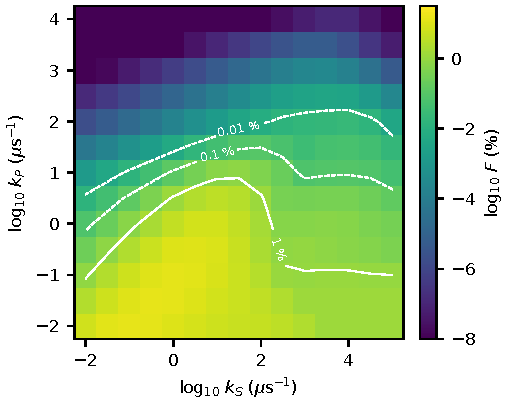
\includegraphics[width=\columnwidth]{fig_map.pdf}
\caption{Largest magnetic field effect on the onward yield found by the search
over the exchange coupling, the field direction and the dipolar scale
$s\in[0,3]$, as a function of the singlet back-transfer rate $k_S$ and the
spin-independent onward rate $k_P$. Reference four-nucleus model, coherent spin
dynamics, $B = 50\,\mu$T.}
\label{fig:map}
\end{figure}

\section{Field effects of a competent pair}

Combining eq~\ref{eq:kmin} with the field effect defines
\begin{equation}
G^*(\Delta) = \sup\{\,F^*(k_S,k_P) : k_S,\,k_P \ge k_{\min}(\Delta)\,\},
\end{equation}
the largest field effect of a pair that can carry the turnover. We evaluate it
by a procedure on the rate grid and call the result $G$. It is not a bound on
$G^*$: between grid points the effect can exceed it. At
$\Delta = \intDelta$~eV, where $k_{\min}$ coincides with the grid rate
$k_P = \intKP~\mu$s$^{-1}$, the permitted point $k_S = \intKS~\mu$s$^{-1}$ gives
\intMFE\,\% against $G = \intG$\,\% (Supporting Information). In the procedure,
$k_{\min}$ is rounded down to the nearest grid rate; above the
largest $k_P$ the edge value is used, because $\max_{k_S}F$ decreases with $k_P$
on the grid, and above the largest $k_S$ only the constraint on $k_P$ is
imposed. Because the permitted region only shrinks as $\Delta$ grows, $G$ is
finally replaced by its running maximum from larger $\Delta$, which removes
non-monotonic steps introduced by these grid rules. Where $k_{\min}$ lies below the grid ($\Delta<\GdefOne$~eV for
$k_{\rm cat}=1$~s$^{-1}$) the grid does not cover the permitted rates, and $G$
is not reported; there slower pairs are permitted and give larger effects.

Figure~\ref{fig:G} shows $G$ for $k_{\rm cat} = 1$--$10^3$~s$^{-1}$. Because
$k_P$ is sampled every half decade, the thresholds below are resolved to about
\gridStep~eV. For $k_{\rm cat}=1$~s$^{-1}$, $G$ falls below 0.1\,\% for
$\Delta\ge\ThrTenthOne$~eV
and below 0.01\,\% for $\Delta\ge\ThrHundredthOne$~eV; for
$k_{\rm cat}=10^3$~s$^{-1}$ the 0.1\,\% threshold is \ThrTenthThousand~eV. A pair
near thermoneutrality is not excluded: at small $\Delta$ competence permits
slow decay and the field effect can be several percent.

\begin{figure}
\centering
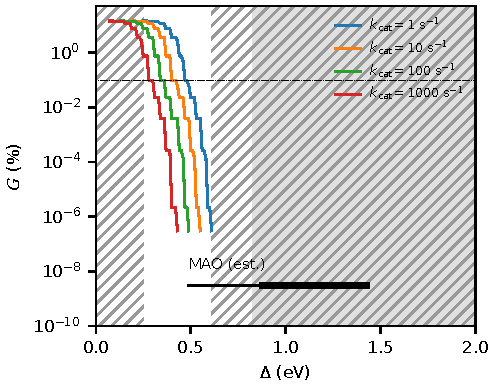
\includegraphics[width=\columnwidth]{fig_G.pdf}
\caption{Largest magnetic field effect found by the grid procedure among
pairs that can carry the turnover, $G(\Delta)$, for $k_{\rm cat} = 1$, 10, 100 and $10^3$~s$^{-1}$ in the
reference model. Hatched: $G$ not defined for $k_{\rm cat}=1$~s$^{-1}$ because
the permitted rates extend below the computed grid. Shaded: no pair carries the turnover with
$\nu_n = 10^{14}$~s$^{-1}$. Bar: driving force of an amine-to-flavin pair in
monoamine oxidase estimated from measured flavin potentials and a proxy amine
potential (Sec.~\ref{sec:mao}).}
\label{fig:G}
\end{figure}

\section{Dependence on the spin model}
\label{sec:sens}

$F$ and $G$ belong to the reference model, and they change with it. We
re-searched the cell that sets the row maximum of $F$ for each onward rate that
determines the thresholds ($k_P = 10$--$10^{2.5}~\mu$s$^{-1}$) in three richer
nuclear models: anisotropic hyperfine tensors for N5 and N10 (density-functional
spin-dipolar parts in the frame of the dipolar tensor), the same with the
aminium $^{14}$N added, and the same with the two largest flavin methyl protons
added. Relative to the reference model the largest factors found are
\XanisoMax\ (anisotropic tensors), \XanisoNMax\ (with $^{14}$N) and
\XanisoHMax\ (with the methyl protons). As a stress test we multiply every
searched value by the largest of these, \Xsens; this shifts the 0.1\,\%
threshold for $k_{\rm cat}=1$~s$^{-1}$ from \ThrTenthOne\ to
\ThrTenthOneSens~eV. Only the reference row-maximum cell was searched again, so
in a richer model another cell of the row could be larger, and the shifted
threshold is the result of a stress test, not an upper bound over spin models.

Electron spin relaxation was computed directly in the four-nucleus model. Every
cell that the thresholds use on these rows ($k_S\ge k_P$, \nTtwoCells\ searches)
was searched again with single-electron dephasing, $T_2^e = 10$~ns, 100~ns and
1~$\mu$s, using a solver that does not build the Liouvillian (Supporting
Information). Relaxation changed individual cells by factors of
\TtwoCellMin--\TtwoCellMax, so it does not reduce $F$ everywhere, but it lowered
every row maximum: the largest value found with relaxation in each row is
\TtwoRowMin--\TtwoRowMax\ times the coherent one. With
each cell replaced by the larger of its coherent and relaxed values, the 0.1\,\%
threshold for $k_{\rm cat}=1$~s$^{-1}$ is \ThrTenthOneRelax~eV and the
0.01\,\% threshold \ThrHundredthOneRelax~eV.

\section{Where monoamine oxidase lies}
\label{sec:mao}

The potentials of the covalent flavin in the monoamine oxidases have been
measured. Chemical reduction proceeds in two steps, the first giving the
semiquinone and each requiring two electron equivalents of the enzyme; the
oxidized/semiquinone midpoint potential is $\EflMAOA$~mV in MAO~A and
$\EflMAOB$~mV in MAO~B,\cite{Sablin2001} and the flavin radical of MAO~A is
anionic,\cite{Kay2007} the radical of the scheme above. We take these midpoints
as the one-electron flavin couple. For the amine, dialkylamine radical cations
in water have $E^\circ({\rm R_2NH^{\bullet+}/R_2NH}) = \EamExp\pm\AmineErr$~V vs
NHE, a value its authors give as a general approximation;\cite{Jonsson1996} we
are not aware of a measured potential for a primary alkylamine or benzylamine
radical cation in water and use this value as a proxy. With the Coulomb
attraction of the contact pair in water (\CoulLo--\CoulHi~eV for 6--3.5~\AA)
this places the pair at $\Delta\approx\DeltaMAOlo$--\DeltaMAOhi~eV.

Substrate binding changes the flavin potential: in the presence of substrates
the midpoint potential for full reduction shifts by up to
$+\SubShift$~V.\cite{Sablin2001} As a bounding assumption, if the one-electron
couple shifted by the same amount, the pair would lie at
$\Delta\approx\DeltaMAOsub$~eV, or \DeltaMAOsubLo--\DeltaMAOsubHi~eV within the
uncertainty of the amine proxy. This range straddles the competence limit of
\DeltaMaxHi~eV, so on this assumption the thermodynamics alone does not
exclude the pair from carrying turnover. It lies, however, well above the
driving forces at which the searched field effect is appreciable ($G<0.1$\,\%
for $\Delta\ge\ThrTenthOne$--\ThrTenthOneSens~eV): a pair at the 0.1\,\%
threshold would require the active site to lower $\Delta$ by a further
$\DeltaToThr$~eV beyond that shift. The kinetic evidence points away from a
long-lived radical pair: no flavin radical is detected during the reductive
half-reaction of MAO~B,\cite{Walker1994} and the substituent and isotope
effects of MAO~A indicate rate-limiting $\alpha$-C--H cleavage by proton
abstraction.\cite{Miller1999} These estimates concern substrates of the
benzylamine type, oxidized at nitrogen. Substrates that may be oxidized at the
ring rather than at nitrogen, such as the catechol and indole
neurotransmitters, are not analysed here and would require their own
potentials.

The electronic coupling between flavin and substrate does not enter
eq~\ref{eq:kmin}, but it indicates the regime. Fragment-orbital couplings for
methylamine at van der Waals contact (\nScanValid\ non-clashing geometries of
\nScan; Supporting Information) are \tContactMed~meV (median) to
\tContactMax~meV at 3.5~\AA, large enough that back electron transfer at contact
would be adiabatic. The reaction terms of eq~\ref{eq:me} are derived for weak,
non-adiabatic coupling.\cite{Fay2018} Eq~\ref{eq:kmin} holds for any generator
of that form with unital, positivity-preserving relaxation, including the
reactive dephasing that appears at higher order; whether a strongly coupled
contact pair is described by such a generator at all is not addressed here, and
$F$ is least reliable for it.

\section{A light-driven pair in the same model}

The flavin--tryptophan pair of cryptochrome is formed by light, so
eq~\ref{eq:kmin} does not apply to it. As a check that the same equations
produce a field response when the rates are not constrained, we evaluated it
with the same scheme and yield observable, averaged over field orientations
rather than maximized, $k_S = k_P = 1~\mu$s$^{-1}$, the pair
1.90~nm apart ($D = \cryDcoup$~MHz), flavin N5 and N10 as above, the two largest
$\beta$-proton couplings (\aTrpOne\ and \aTrpTwo~MHz) and N1 of the tryptophan
radical cation from the same density-functional method, and the exchange
coupling on \nCry\ values spanning the literature range of its prefactor with
both signs.\cite{Efimova2008} The orientation-averaged response ranges from
below $10^{-2}$\,\% (it changes sign within the range) to \cryMax\,\%. This is
a numerical control, not a like-for-like comparison: the hyperfine couplings,
dipolar coupling and rates differ from the enzyme model as well as the way the
pair is formed.

\section{Discussion}

The bound of eq~\ref{eq:kmin} applies to any radical pair that is formed
thermally from a closed-shell state, returns to it only through the singlet,
and carries the catalytic flux; a pair on a dead-end branch is limited instead
by the population bound of the same section. Both require the reaction terms of
eq~\ref{eq:me} and unital, positivity-preserving relaxation, but no electronic
coupling, reorganization energy or particular onward chemistry. The numbers that
follow depend on more: $F$ and $G$ are the results of a finite search in a
specific spin model with coherent dynamics, the shifted threshold is a stress
test, and the monoamine oxidase estimate depends on a dialkylamine potential
standing in for the substrates and on how substrate binding shifts the
one-electron flavin couple.

Two routes around the bound should be named. Three-radical and scavenging
mechanisms\cite{Kattnig2017} restore sensitivity to strongly coupled pairs; they
still require the pair to survive until the third radical acts, which
eq~\ref{eq:kmin} limits, but their field effects would have to be computed in
their own model. And an active site that brings $\Delta$ close to zero is not
excluded: competence then allows slow decay and field effects of a percent or
more. The question for a particular enzyme is where its radical pair lies in
$\Delta$, which is measurable.

\section{Conclusions}

For a radical pair that an enzyme forms thermally and through which it turns
over, detailed balance bounds the singlet back-transfer rate and the
spin-independent onward rate from below by $k_{\rm cat}e^{\Delta/k_BT}$, for any
spin Hamiltonian and unital, positivity-preserving relaxation. In a
flavin--aminium spin model with computed hyperfine and dipolar couplings, the
largest field effect found among the searched pairs that can carry
$k_{\rm cat}=1$~s$^{-1}$ falls below 0.1\,\% for $\Delta\ge\ThrTenthOne$~eV
(\ThrTenthOneSens~eV in a stress test for richer nuclear models, and
\ThrTenthOneRelax~eV with electron spin relaxation included). The measured
flavin potentials of the monoamine oxidases, with a dialkylamine proxy for the
potential of benzylamine-type substrates, place an amine-to-flavin pair at
\DeltaMAOsubLo--\DeltaMAOhi~eV, depending on how substrate binding shifts the
one-electron couple, above that range.

\section*{Supplementary Material}
See the supplementary material for the 300-system test of
eq~\ref{eq:phibound}, the full search results, the electron-spin-relaxation
calculations in the four-nucleus model, the hyperfine and dipolar tensors, the
coupling scan, the density-functional driving forces, the model-sensitivity
calculations, the cryptochrome scan, and software and environment.

\section*{Author Declarations}
\subsection*{Conflict of Interest}
The authors have no conflicts to disclose.
\subsection*{Author Contributions}
\textbf{Hikaru Wakaura:} Conceptualization (lead); Methodology (lead); Software
(lead); Validation (lead); Formal analysis (lead); Investigation (lead); Data
curation (lead); Visualization (lead); Writing -- original draft (lead);
Writing -- review \& editing (lead). \textbf{Taiki Tanimae:} Supervision
(lead).

\section*{Data Availability}
The data that support the findings of this study and the code that generates
them are openly available in the \texttt{qbscreen} package at
\url{https://github.com/deeptell-inc/brain_protein_screening}; every number in
the text is generated from the stored results by
\texttt{qbscreen/make\_numbers\_v6.py}.

\bibliography{refs}

\end{document}
